\section{Signal extraction and limit setting}\label{chap6:SignalExtractionAndLimits}

The signal yield, including both ggH and VBF production modes, is extracted performing a combined fit of the three categories to the \mti simulation templates for backgrounds and signal, and is repeated for each resonance mass hypothesis. Moreover, fixed the mass of the resonance, the fit is performed again for the various hypotheses of the resonance decay width. A single signal strength $\mu$ is extracted from each fit, which multiplies both the ggH and VBF contributions. In other words it is assumed that the ratio of the two production mechanism stays the same as the one predicted by the SM\footnote{This is an approximation that limits the amount of models that can be tested with the provided results. A future development of this analysis, with larger integrated luminosity, might also include the cases for which different ggH and VBF relative contributions are expected.}.

The background yields expected from simulation corresponding to the three jet categories and after the analysis event selection are shown in Table~\ref{tab:bkg_yields}. The signal yields corresponding to a selection of mass points and assuming $\Gamma' = \Gamma_\mathrm{SM}$ are shown in Table~\ref{tab:sig_yields}.

\begin{table}[htb]
\begin{center}
\caption{Expected yields estimated from simulation (except for the non-prompt contribution which is estimated using data) for each background process in the three analysis categories, after the analysis event selection. The uncertainties are shown for the processes estimated from simulation.}\label{tab:bkg_yields}
\small{
\begin{tabular}{c c c c }
\toprule
             Background process           &         0 jets                                          &          1 jet                                         &        VBF                                           \\
\midrule
      qq$\to$WW                &    501.93 $\pm$       0.00 (0\%)              &     198.72 $\pm$       0.00 (0\%)             &      4.54 $\pm$       0.00 (0\%)               \\
      gg$\to$WW                &     37.28 $\pm$       5.77 (15\%)              &      19.63 $\pm$       3.04 (15\%)             &      1.05 $\pm$       0.16 (15\%)               \\
      Top quark                &    188.75 $\pm$       0.00 (0\%)              &     330.05 $\pm$       0.00 (0\%)             &     25.06 $\pm$       0.00 (0\%)               \\
      DY                &     33.24 $\pm$       0.00 (0\%)              &      12.99 $\pm$       0.00 (0\%)             &      0.28 $\pm$       0.00 (0\%)               \\
      Non-prompt                &     64.21 $\pm$      19.26 (30\%)              &      31.69 $\pm$       9.51 (30\%)             &      2.10 $\pm$       0.63 (30\%)               \\
      V$\gamma$                &     26.62 $\pm$       0.72  (3\%)              &      14.18 $\pm$       0.38  (3\%)             &      0.64 $\pm$       0.02 (3\%)               \\
     V$\gamma^*$                &      4.44 $\pm$       1.12 (25\%)              &       3.39 $\pm$       0.85 (25\%)             &      0.14 $\pm$       0.04 (25\%)               \\
     VZ                &     13.51 $\pm$       0.76  (6\%)              &      11.67 $\pm$       0.66 (6\%)             &      0.28 $\pm$       0.02 (6\%)               \\
     VVV                &      0.01 $\pm$       0.00 (3\%)              &       0.02 $\pm$       0.00 (3\%)             &      0.00 $\pm$       0.00 (3\%)               \\   
     
 SM H$\to$WW           &      6.04 $\pm$       0.40  (7\%)              &       3.10 $\pm$       0.11 (5\%)             &      0.34 $\pm$       0.02 (7\%)               \\
 
 SM H$\to\tau\tau$                &      0.50 $\pm$       0.05 (9\%)              &       0.43 $\pm$       0.04 (9\%)             &      0.04 $\pm$       0.00 (9\%)               \\
      
\midrule
    Total background          &    876.5               &     625.9           &     34.5          \\
\bottomrule
\end{tabular}
}
\end{center}
\end{table}

\begin{table}[htb]
\begin{center}
\caption{Expected signal yields for the ggH and VBF production modes estimated from simulation after the analysis event selection for different mass hypothesis assuming $\Gamma' = \Gamma_\mathrm{SM}$ in the three analysis categories. The errors correspond to the theoretical uncertainties in the signal estimation.}\label{tab:sig_yields}
\small{\begin{tabular}{c c c c } 
\toprule
                 Mass [GeV]                 &          0 jets    &          1 jet              & VBF           \\ 
\midrule
\multicolumn{4}{c}{ggH signal yields} \\
\midrule
 200                        &      90.21 $\pm$       6.67 (7\%)             &      37.47 $\pm$       1.81 (5\%)     &       1.25 $\pm$       0.26 (21\%)      \\
 400                        &      66.35 $\pm$       4.90 (7\%)             &      32.65 $\pm$       1.57 (5\%)     &       2.04 $\pm$       0.42 (21\%)      \\
 600                        &      13.86 $\pm$       1.05 (8\%)             &       8.56 $\pm$       0.44 (5\%)     &       0.68 $\pm$       0.14 (21\%)      \\
 800                        &       3.20 $\pm$       0.25 (8\%)             &       2.32 $\pm$       0.13 (6\%)     &       0.22 $\pm$       0.05 (21\%)      \\
 1000                       &       0.88 $\pm$       0.07 (8\%)             &       0.70 $\pm$       0.04 (6\%)     &       0.07 $\pm$       0.02 (21\%)      \\
\midrule
\multicolumn{4}{c}{VBF signal yields} \\
\midrule
 200                        &       1.54 $\pm$       0.06 (4\%)             &       6.18 $\pm$       0.25 (4\%)     &       5.05 $\pm$       0.20 (4\%)      \\
 400                        &       0.91 $\pm$       0.04 (4\%)             &       3.42 $\pm$       0.14 (4\%)     &       3.19 $\pm$       0.13 (4\%)      \\
 600                        &       0.50 $\pm$       0.02 (4\%)             &       1.95 $\pm$       0.08 (4\%)     &       1.88 $\pm$       0.08 (4\%)      \\
 800                        &       0.33 $\pm$       0.01 (4\%)             &       1.21 $\pm$       0.05 (4\%)     &       1.16 $\pm$       0.05 (4\%)      \\
 1000                       &       0.22 $\pm$       0.01 (4\%)             &       0.79 $\pm$       0.03 (4\%)     &       0.69 $\pm$       0.03 (4\%)      \\
\bottomrule
\end{tabular}
}
\end{center}
\end{table}

The strategy for computing the exclusion limits is based on the modified frequentist approach, also referred to as $\mathrm{CL_s}$, as described in~\cite{CMS-NOTE-2011-005}. The first step is to construct the likelihood function $\mathcal{L}(\mu,\theta)$:
\begin{equation}
\mathcal{L}(\mu,\theta) = Poisson(data|\mu\cdot s(\theta) + b(\theta))\cdot p(\tilde{\theta}|\theta) \quad,
\end{equation}
where $data$ represents the experimental observation, $s$ and $b$ are the expected signal and background yields respectively and $\theta$ is the full set of true values for the nuisance parameters constrained by the prior distribution functions $p(\tilde{\theta}|\theta)$. The default values assigned to the nuisance parameters are labelled as $\tilde{\theta}$.

For a binned shape analysis, $Poisson(data|\mu\cdot s + b)$ is the product of the Poisson probabilities to observe $n_i$ events in bin i:
\begin{equation}
\prod_i \frac{(\mu\cdot s_i + b_i)^{n_i}}{n_i !} e^{-\mu\cdot s_i - b_i} \quad.
\end{equation}
In order to test the compatibility of the data with the signal plus background (or the background only) hypothesis, the test statistic $\tilde{q}_\mu$ is constructed based on the profile likelihood ratio:
\begin{equation}
\tilde{q}_\mu = -2 \ln{\frac{\mathcal{L}(data|\mu,\hat{\theta}_\mu)}{\mathcal{L}(data|\hat{\mu},\hat{\theta})	}}  \quad \mathrm{with} \quad 0 \leq \hat{\mu} \leq \mu \quad ,
\end{equation}
where $\hat{\theta}_\mu$ refers to the conditional maximum likelihood estimators of $\theta$, given the signal strength $\mu$. The parameter estimators $\hat{\mu}$ and $\hat{\theta}$ correspond to the global maximum of the likelihood. The $0 \leq \hat{\mu}$ constraint is imposed to have a positive signal yield, e.g. background underfluctuations are forbidden, while $\hat{\mu} \leq \mu$ is imposed to have a one-sided confidence interval. The observed test statistic for the signal strength $\mu$ under test is referred to as $\tilde{q}_\mu^\mathrm{obs}$. The values of the nuisance parameters obtained maximising the likelihood function are labelled as $\hat{\theta}_0^\mathrm{obs}$ and $\hat{\theta}_\mu^\mathrm{obs}$ for the background only and signal plus background hypotheses, respectively. The pdf of the test statistic in constructed by generating toy MC pseudo-data for both the background only and signal plus background hypotheses, i.e. $f(\tilde{q}_\mu|\mu,\hat{\theta}_\mu^\mathrm{obs})$ and $f(\tilde{q}_\mu|0,\hat{\theta}_0^\mathrm{obs})$. These distributions can be used to define two p-values corresponding to the two hypotheses, $p_\mu$ and $p_b$:
\begin{equation}
p_\mu = P(\tilde{q}_\mu \geq \tilde{q}_\mu^\mathrm{obs}|\mathrm{signal+background}) = \int_{\tilde{q}_\mu^\mathrm{obs}}^{\infty} f(\tilde{q}_\mu|\mu,\hat{\theta}_\mu^\mathrm{obs}) d\tilde{q}_\mu \quad ,
\end{equation}
\begin{equation}
1 - p_b = (\tilde{q}_\mu \geq \tilde{q}_\mu^\mathrm{obs}|\mathrm{background~only}) = \int_{\tilde{q}_0^\mathrm{obs}}^{\infty} f(\tilde{q}_\mu|0,\hat{\theta}_0^\mathrm{obs}) d\tilde{q}_\mu \quad .
\end{equation}
According to these definitions, $p_\mu$ and $p_b$ can be identified with $\mathrm{CL_{s+b}}$ and $1-\mathrm{CL_b}$, respectively.
The $\mathrm{CL_s}(\mu)$ is calculated using the following ratio:
\begin{equation}
\mathrm{CL_s}(\mu) = \frac{\mathrm{CL_{s+b}}}{\mathrm{CL_b}} = \frac{p_\mu}{1-p_b} \quad .
\end{equation}
If, for a given signal strength $\mu$, $\mathrm{CL_s} \leq \alpha$, then the hypothesis is excluded with a $(1-\alpha)$ confidence level (CL). For instance, if one wants to quote the upper limit on $\mu$ with a 95\% CL, the signal strength has to be adjusted until $\mathrm{CL_s} = 0.05$.

The expected median upper limit, as well as the $\pm 1\sigma$ (68\% CL) and $\pm 2\sigma$ (95\% CL) bands, are determined generating a large amount of pseudo-data in the background only hypothesis and calculating $\mathrm{CL_s}$ and the 95\% CL upper limit for each of them, as if they were real data. Then the cumulative distribution of the 95\% CL upper limits is built and the median expected value is identified as the value at which the cumulative distribution crosses the 50\% quantile. The $\pm 1\sigma$ ($\pm 2 \sigma$) band is defined by the values at which the cumulative distribution crosses the 16\% (2.5\%) and 84\% (97.5\%) quantiles.

In order to assess the sensitivity of the analysis, the expected upper exclusion limits at 95\% CL on the signal strength are shown in Fig.~\ref{fig:13TeVexplim} for the three jet categories separately. For a given mass of the resonance, the limits are derived assuming a signal decay width $\Gamma' = \Gamma_\mathrm{SM}$ and a cross section equal to the one expected from a SM Higgs boson at that mass. The other decay width hypotheses have been tested as well, showing a very similar expected exclusion limit, suggesting that this analysis is not strongly sensitive to variations of the resonance decay width. In fact, the width of the \mti distribution is driven by the experimental resolution and the choice of different decay widths has a mild effect on this variable.

The 0 jets category is the most sensitive especially in the low mass region, while for very large masses of the resonance the 1 jet and VBF categories start being important. This is explained mainly by the fact that the VBF contribution increases, with respect to ggH, as the mass increases. The expected exclusion limit on the signal strength after the combination of the three categories is shown in Fig.~\ref{fig:13TeVcombexplim}. Comparing the limits in the single categories with the combination of the three it is evident how the higher jet multiplicity categories help in improving the results for large values of $M_\mathrm{X}$. For the analysed luminosity the expected exclusion mass range for the production of a resonance with the SM Higgs boson cross section extends roughly from 350 to 450\GeV.

\begin{figure}[!htb]
\centering
\subfigure[0 jets]{
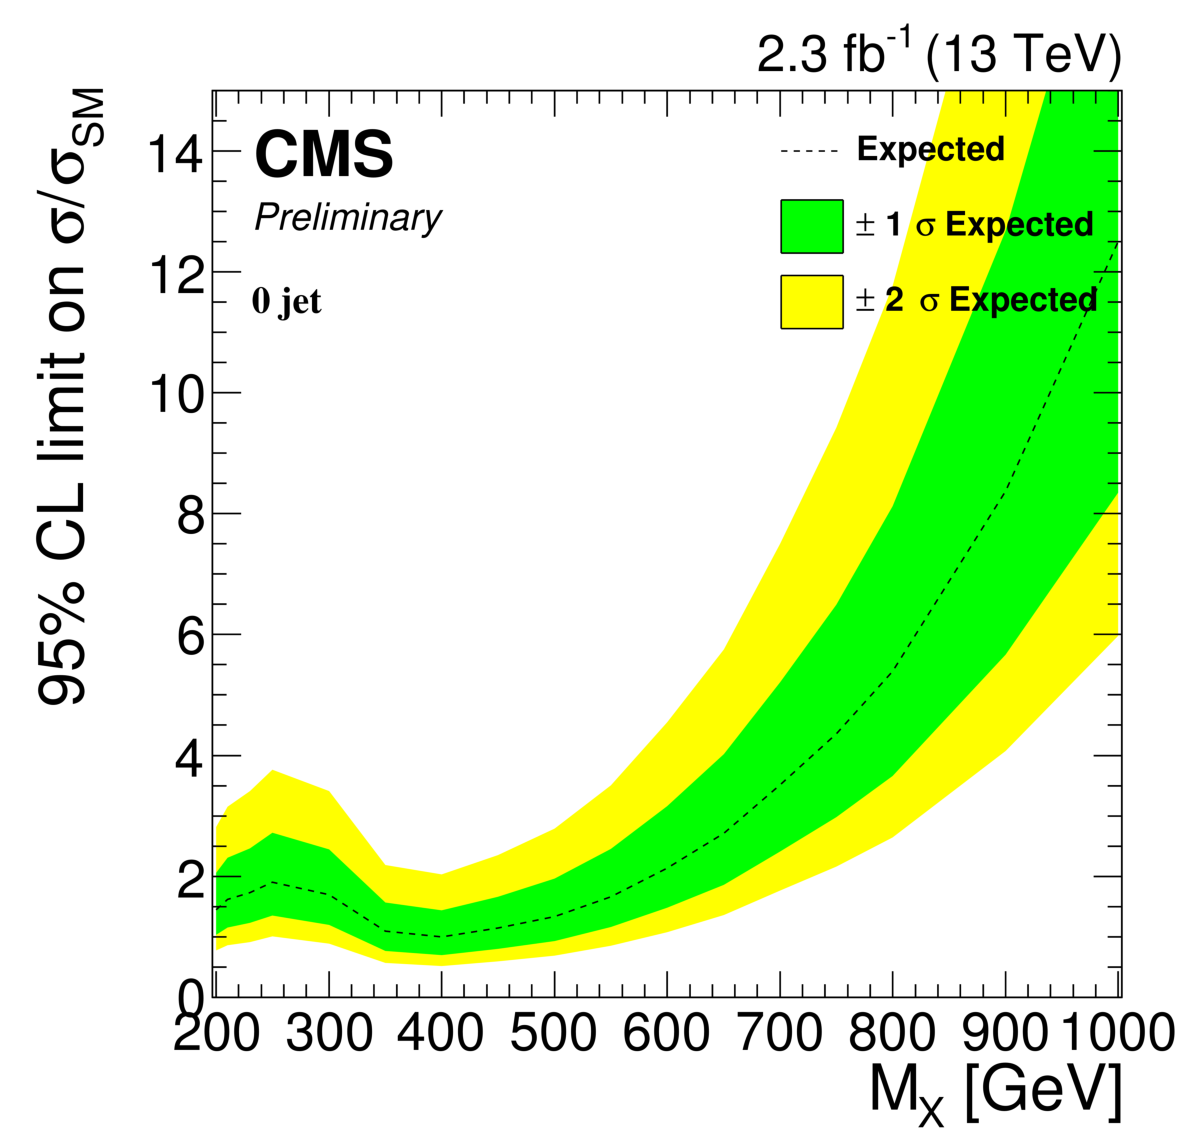
\includegraphics[width=0.31\textwidth]{images/13TeV/HighMass/exp_limit_0jet_mu.pdf}
}
\subfigure[1 jet]{
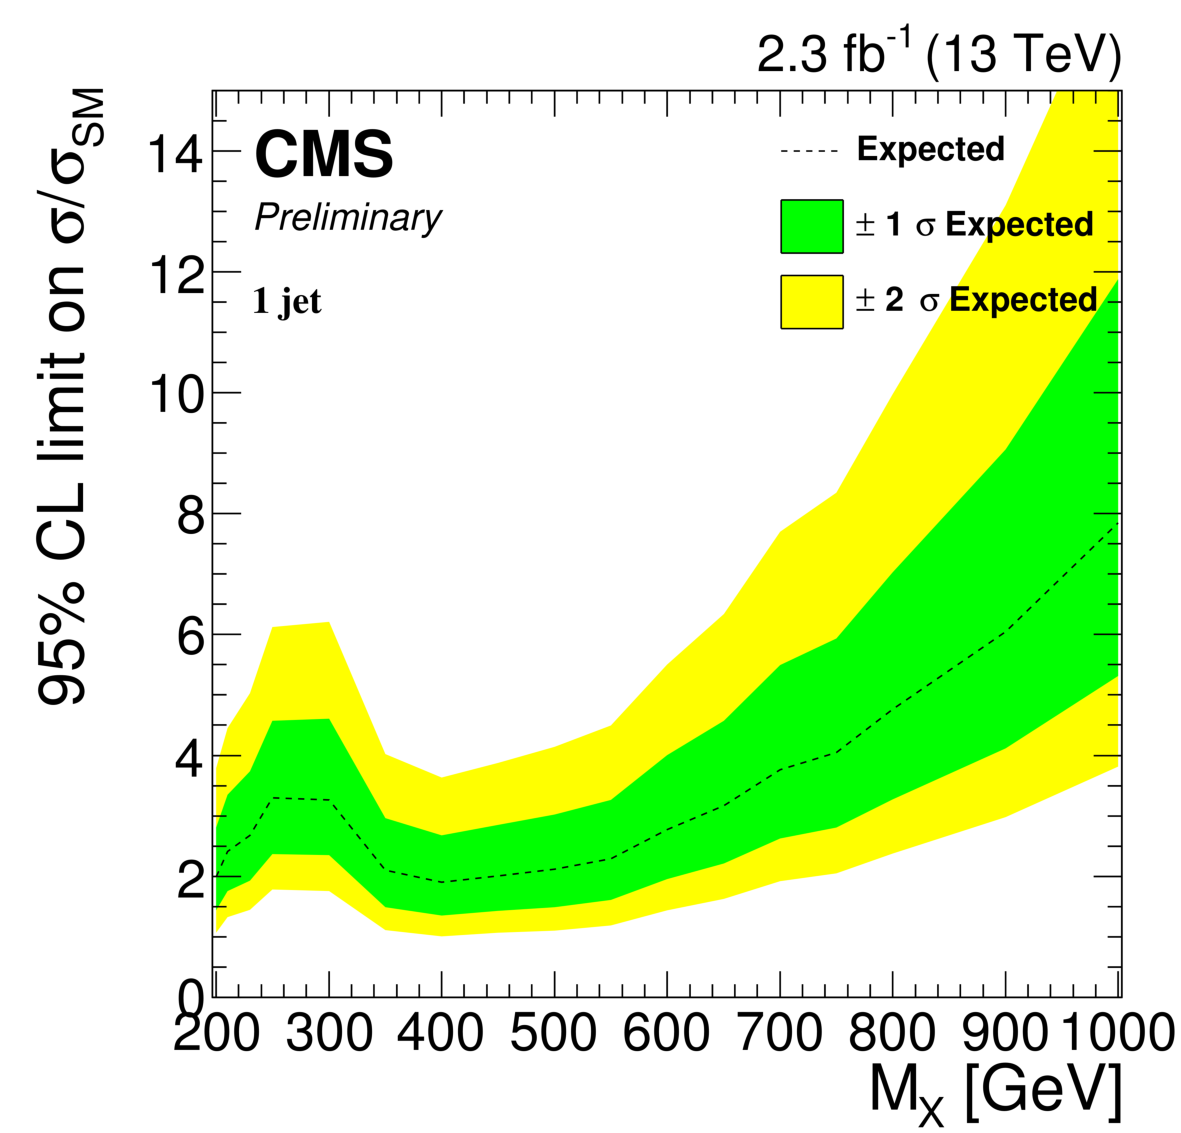
\includegraphics[width=0.31\textwidth]{images/13TeV/HighMass/exp_limit_1jet_mu.pdf}
}
\subfigure[2 jets]{
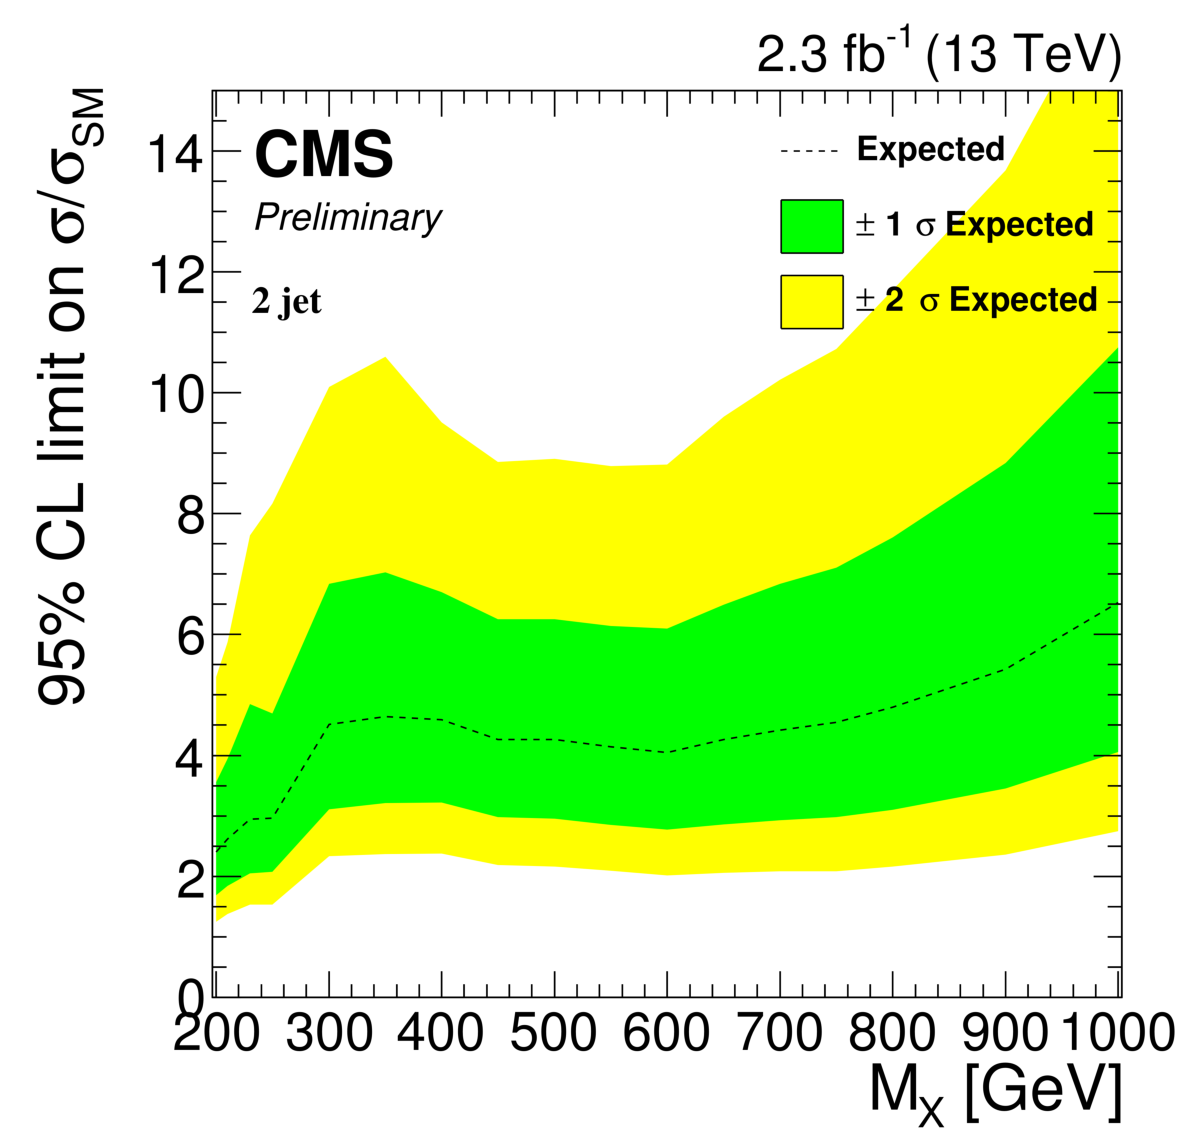
\includegraphics[width=0.31\textwidth]{images/13TeV/HighMass/exp_limit_2jet_mu.pdf}
}
\caption{Expected exclusion upper limits at 95\% CL on the signal strength in the three categories, as a function of the resonance mass. The dashed line corresponds to median upper limit, while the green and yellow regions represent the $\pm 1\sigma$ and $\pm 2 \sigma$ uncertainty bands, respectively. Limits are derived assuming the SM Higgs boson cross section and decay width for each mass point.}\label{fig:13TeVexplim}
\end{figure}

\begin{figure}[!htb]
\centering
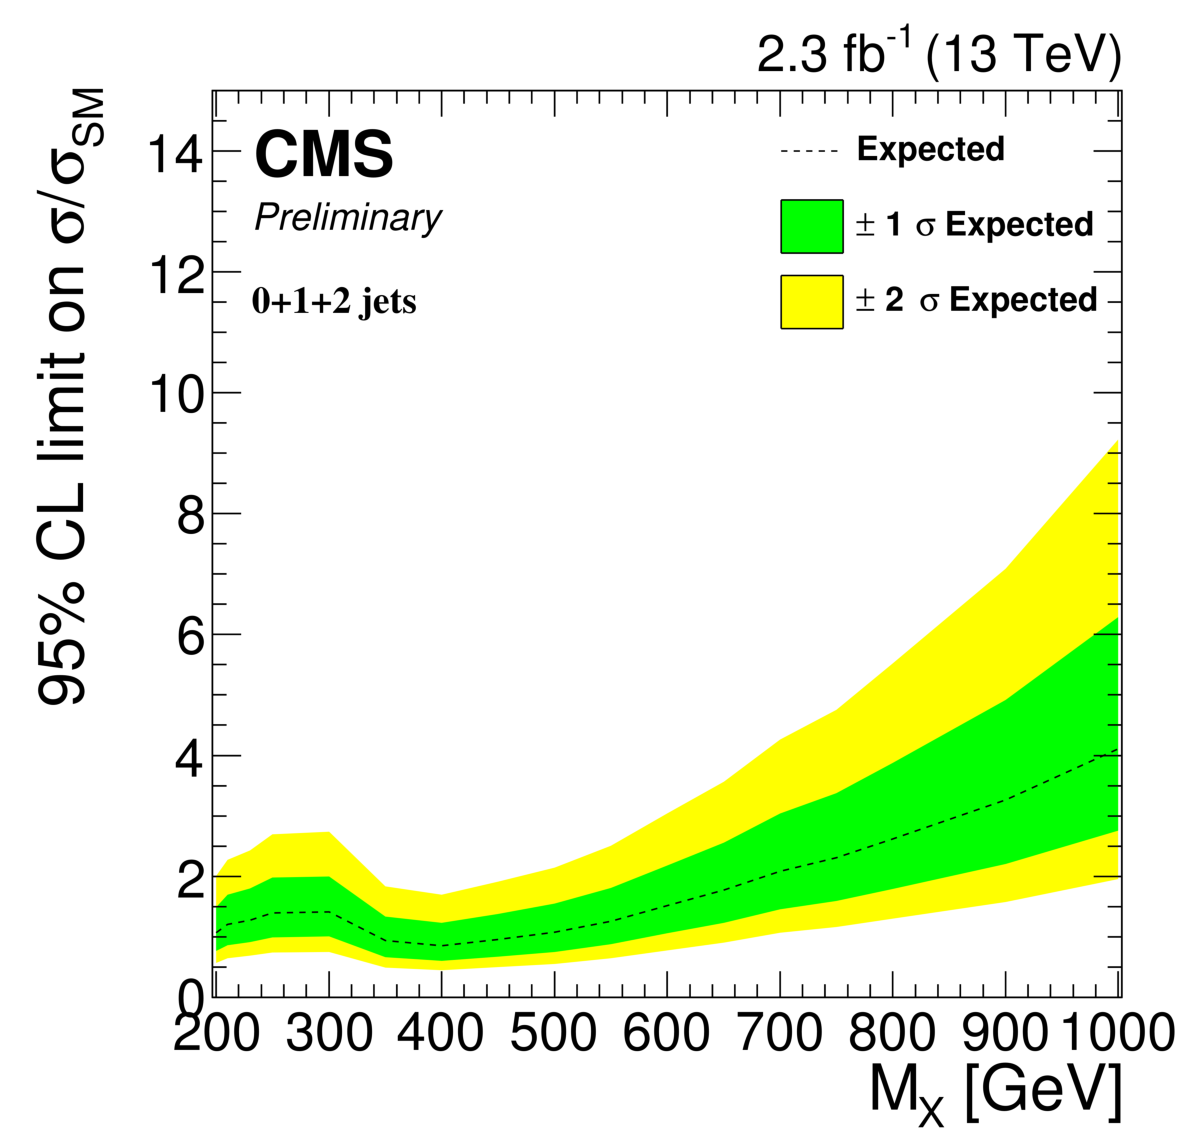
\includegraphics[width=0.5\textwidth]{images/13TeV/HighMass/exp_limit_012jet_mu.pdf}
\caption{Expected exclusion upper limit at 95\% CL on the signal strength for the combination of the three categories, as a function of the resonance mass. The dashed line corresponds to median upper limit, while the green and yellow regions represent the $\pm 1\sigma$ and $\pm 2 \sigma$ uncertainty bands, respectively. The limit is derived assuming the SM Higgs boson cross section and decay width for each mass point.}\label{fig:13TeVcombexplim}
\end{figure}



